\documentclass[mathserif]{beamer} 
\usepackage{eulervm} %красивый математический шрифт - по желанию
\usepackage{ulem} %зачёркивания
\usepackage{bm} %особо жирный математический
\usepackage{schemata} %для красивых блочных переходов, пользуюсь редко
\usepackage{mathtools} %улучшенная работа с типографией в math mode
\setbeamertemplate{navigation symbols}{} %отключает управляющие символы в правом нижнем углу
\usefonttheme{professionalfonts}
\usepackage{cmap} %чтобы были работающие гиперссылки
\usepackage{makeidx,fancybox,tikz}
\usetikzlibrary{automata, positioning, arrows,patterns}
\usetikzlibrary{arrows.meta}
\usepackage{tempora} %по желанию -- русские штрифты с засечками

\mode<presentation>
{
  \usetheme{CambridgeUS}
  \usecolortheme{dove} 
}
\usepackage[T1,T2A]{fontenc}
\usepackage[utf8]{inputenc}
\usepackage[english,russian]{babel}
\usepackage{amsmath,mathrsfs} %ещё больше математических символов
\usepackage{amstext}
\usepackage{graphicx,relsize}
\graphicspath{ {./../images/} }

\usepackage{color}
\definecolor{gray}{rgb}{0.4,.4,0.4} %здесь можно определить собственные цвета
\definecolor{grey80}{rgb}{0.8,.8,0.8}
\definecolor{grey90}{rgb}{0.9,.9,0.9}
\definecolor{grey95}{rgb}{0.95,.95,0.95}
\newcommand\redstroke{\bgroup\markoverwith
{\textcolor{red}{\rule[0.5ex]{2pt}{1.5pt}}}\ULon} %зачёркивание жирной красной чертой

\newcommand\reduline{\bgroup\markoverwith
{\textcolor{red}{\rule[-0.5ex]{2pt}{1.5pt}}}\ULon}%подчёркивание жирной красной чертой

\newcommand\bluline{\bgroup\markoverwith
{\textcolor{blue}{\rule[-0.5ex]{2pt}{1.5pt}}}\ULon}

\newcommand\bolduline{\bgroup\markoverwith
{\textcolor{white}{\rule[-0.5ex]{2pt}{1.5pt}}}\ULon}

\title[] {Автомат Антимирова}

\author[Chipollino]{Лучшая команда разработчиков по ТФЯ} % :))
\date[] 
{2022 г.}
\subject{Computer Science}

\newcommand{\Lang}{\mathscr{L}} %макрос для языка регулярки или автомата
\def\logor{\mathrel{\vee}} %отрендеренные логические операторы (с правильными интервалами)
\def\logimpl{\mathrel{\Rightarrow}}
\def\Linearize{\mathtt{Linearize}} %названия операций интерпретатора записываем моноширинным
\def\First{\mathrm{First}} %названия прочих операций записываем обычным шрифтом, но не тем, который в math mode по умолчанию
\def\Last{\mathrm{Last}}
\def\Follow{\mathrm{Follow}}
\def\IlieYu{\mathrm{IlieYu}}
\def\Glushkov{\mathtt{Glushkov}}
\def\Thompson{\mathtt{Thompson}}
\def\Antimirov{\mathtt{Antimirov}}
\def\RemEps{\mathtt{RemEps}}
\def\DeAnnote{\mathtt{DeAnnote}}
\def\Annote{\mathtt{Annote}}
\def\Minimize{\mathtt{Minimize}}
\def\logand{\mathrel{\&}}
\def\lognot{\mathop{\neg}}
\def\iff{\mathrel{\Leftrightarrow}}
\def\quantall#1{\mathop{\forall #1}}
\def\quantex#1{\mathop{\exists #1}} 
\def\alter{\ensuremath{\mathrel{\vert}}}%отрендеренные регулярные операторы 
\def\star{\ensuremath{^{*}}}%отрендеренные регулярные операторы 
\def\regexpstr#1{\mathtt{#1}}%буквы внутри регулярок переписываются в моноширинный
\newcommand{\Nat}{\mathbb N}
\newcommand{\empt}{\varepsilon} %пустое слово
\newcommand{\bottom}{\bot} %противоречие
\newcommand{\rar}{\rightarrow} %стрелка вправо. Для экономии букв.
\newcommand{\RegExp}{\mathcal{RE}} %макрос для обозначения множества всех регулярок
%в преамбулу можно и нужно добавлять свои макросы

\begin{document}

\maketitle
% descriptive documentation : section
\section{Основные понятия}
\begin{frame}{Частичные производные}
    \vspace{-5pt}
    $\alpha_{c}(R)$ — это регулярное выражение $R'$ такое, что если $w \in \Lang(R')$, то $cw \in \Lang(R)$. Обратное не обязательно выполняется. Вычислить частичные производные можно по следующему рекурсивному алгоритму.
    \[\alpha_{c}(c) = \{\empt\}\] % the Derivative placeholder 1 % the Derivative placeholder displaystyle
    \[\alpha_{c}(c') = \varnothing\] % the Derivative placeholder 2 % the Derivative placeholder displaystyle
    \[\alpha_{c}(\empt) = \varnothing\] % the Derivative placeholder 3 % the Derivative placeholder displaystyle
    \begin{equation*}
        \alpha_{c}(r_{1} r_{2}) =
        \begin{cases}
            \{r r_{2} | r \in \alpha_{c}(r_{1})\} \cup \alpha_{c}(r_{2}) & \text {если} \empt \in \Lang(r_{1}) \\ % the Derivative placeholder 4 % the Derivative placeholder displaystyle
            \{r r_{2} | r \in \alpha_{c}(r_{1})\}                        & \text {иначе}                       % the Derivative placeholder 5 % the Derivative placeholder displaystyle
        \end{cases}
    \end{equation*}
    \[\alpha_{c}(\bot) = \varnothing\] % the Derivative placeholder 6 % the Derivative placeholder displaystyle
    \[\alpha_{c}(r_{1}|r_{2}) = \alpha_{c}(r_{1}) \cup \alpha_{c}(r_{2})\] % the Derivative placeholder 7 % the Derivative placeholder displaystyle
    \[\alpha_{c}(r\star) = \{r'r\star | r' \in \alpha_{c}(r)\}\] % the Derivative placeholder 8 % the Derivative placeholder displaystyle
    Автомат Антимирова аналогичен автомату Брзозовски, но состояния представляют собой элементы $\alpha_{w}$, а не $\delta_{w}$. Упрощать по ACI состояния не требуется — их множество и так конечно.
\end{frame} % descriptive documentation

\section{Автомат Антимирова}
\begin{frame}{Пример автомата Антимирова}
    \vspace{-5pt}
    Положим $R_{1} = (\regexpstr{ab} \alter \regexpstr{b})\star \regexpstr{ba}$. % the initial regexp placeholder

    Тогда (производные, равные пустому множеству, здесь опущены):\\
    $\alpha_{a}(R_{1}) = \{\regexpstr{b}(\regexpstr{b}\alter \regexpstr{b})\star\regexpstr{ba}\}$ -- положим $R_{2} = \regexpstr{b}(\regexpstr{ab}\alter \regexpstr{b})\star\regexpstr{ba}$\\  % the Derivative placeholder 1
    $\alpha_{b}(R_{1}) = \{(\regexpstr{ab}\alter \regexpstr{b})\star\regexpstr{ba}, \regexpstr{a}\}$ -- положим $R_{3} = \regexpstr{a}$\\  % the Derivative placeholder 2
    $\alpha_{b}(R_{2}) = \{(\regexpstr{ab}\alter \regexpstr{b})\star \regexpstr{ba}\}$ -- тут ничего нового\\  % the Derivative placeholder 3
    $\alpha_{a}(R_{3}) = \{\empt\}$ — положим $R_{4} = \empt$\\  % the Derivative placeholder 4
    Соответствующий автомат имеет состояния $R_{i}$ и один недетерминированный переход.

    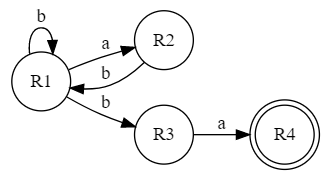
\includegraphics[width=2in, keepaspectratio]{antimirov1.png} % the Antimirov diagram placeholder
\end{frame}

% overall documentation : section 
\section{Обсуждение}
\begin{frame}{Дополнительные сведения}
    \begin{block}{\bf Связь с автоматом Томпсона}
        Автомат Антимирова может быть получен из автомата Томпсона путем последовательного применения к нему следующих операций:
        \[\RemEps(\DeAnnote(\Minimize(\RemEps(\Annote(\Thompson(r))))))\] % the formula Antimirov placeholder displaystyle
    \end{block}
    \begin{block}{\bf Теорема}
        Пусть $r$ -- взвешенное регулярное выражение над $K$. Если $K$ является $null-k$-замкнутым для $r$, то $\Antimirov(r)$ может быть вычислен за $O(m log m + mn)$ путем применения удаления $\empt$-переходов и минимизации.
    \end{block}
    Мы будем говорить, что $K$ является $null-k$-замкнутым для $\alpha$, если $\exists k \geq 0$, такое, что для каждого подтерма $\beta^*$ $null(\beta)^* = \oplus_{i=0}^{k} null(\beta)^i$.
\end{frame}
\end{document}
